\section{Optimal Control}
\label{sec:methods:control}

From a general perspective, the state-estimation methods discussed in the previous section transform one temporal sequence into another. These two sequences are related through the underlying dynamical system. The same perspective also applies to the control framework: in an \ac{MPC} setting, the simulation model maps the current state and control input to the next state; a control policy finds the next control input from the target and observations; a path planner generates a sequence of future control inputs from the current state and the relevant history. In this section, we will discuss how to integrate the normalizing-flow-based methods into control frameworks.

The four methods are applied differently in a control framework due to their different characteristics. 
\begin{enumerate}
    \item \textbf{AmortizedSeqFlow} is based on training a desired mapping offline and then directly using the trained model online. Thus, the optimization process of finding the optimal control input is performed implicitly offline by training the posterior of control inputs conditioned on the observed and reference signals. Once trained, the control input can be inferred directly. Thus, it is approprate to use AmortizedSeqFlow to replace the optimization loop in a standard \ac{MPC} framework.
    \item \textbf{LatentSSMFlow} applies a linear state space model in the latent space, which is natural to adapt it to capturing the underlying dynamics of the system. The system states are then modeled stochastically by taking the previous states and inputs as conditions, i.e., $\boldsymbol{x}_t \leftarrow (\boldsymbol{x}_{t-1}, \boldsymbol{u}_{t-1})$. Then, the control input is optimized in a stochastic \ac{MPC} framework.
    \item \textbf{NormFlowSDE}, likewise, can also model the system dynamics and be integrated into a stochastic \ac{MPC} framework, such as \ac{MPPI}.
    \item \textbf{CondStochInterpolant} is a conditional generative model, which can be used as a control policy or path planner to generate sequential control inputs conditioned on the current system states and observation histories. We compare its performance with \ac{DDPO} \citep{black2024trainingdiffusionmodelsreinforcement}.
\end{enumerate}

Due to the different characteristics and the modeling capabilities of the four methods, they are also validated with different experiments, which are suitable for their respective control frameworks as well.

\subsection{AmortizedSeqFlow in MPC}
Recall the Section~\ref{sec:mpc}, a standard \ac{MPC} requires solving a constrained trajectory optimization problem at every single environment time step. This is highly compute-intensive and can cause execution latencies. At every time step for updating the system, a sequence of future control inputs are supposed to be optimized based on the observed and referred signals. This mapping from observations and references to control inputs can be learned by the AmortizedSeqFlow. It bypasses this iterative optimization loop entirely and effectively "amortizes" the optimization cost.

As shown in Figure~\ref{fig:amortized_seq_flow_control}, the whole \ac{MPC} block including the optimization and model, together with the state estimation are replaced by a two-head conditional normalizing flow. One head extracts information from the reference signals, while the other head is a similar condition network for the history observations. The normalizing flow transforms a latent sequence to the control input sequence under the conditions from both heads. In this setting, only the average input sequence is applied and the posterior uncertainty is not considered.

Once the action chunk $\boldsymbol{u}_{0:H-1}$ is generated, the first control action $\boldsymbol{u}_{0}$ is extracted and applied to the system (the physical robot or plant). The system interacts with environmental disturbances/noise $\epsilon$ and advances one step, producing a new observation $\boldsymbol{y}_1$. The history buffer is then updated ($\boldsymbol{y}_{...:0}\rightarrow [\boldsymbol{y}_{...:0},\boldsymbol{y}_1]$) and ready for the next control cycle.

\begin{figure}
\centering
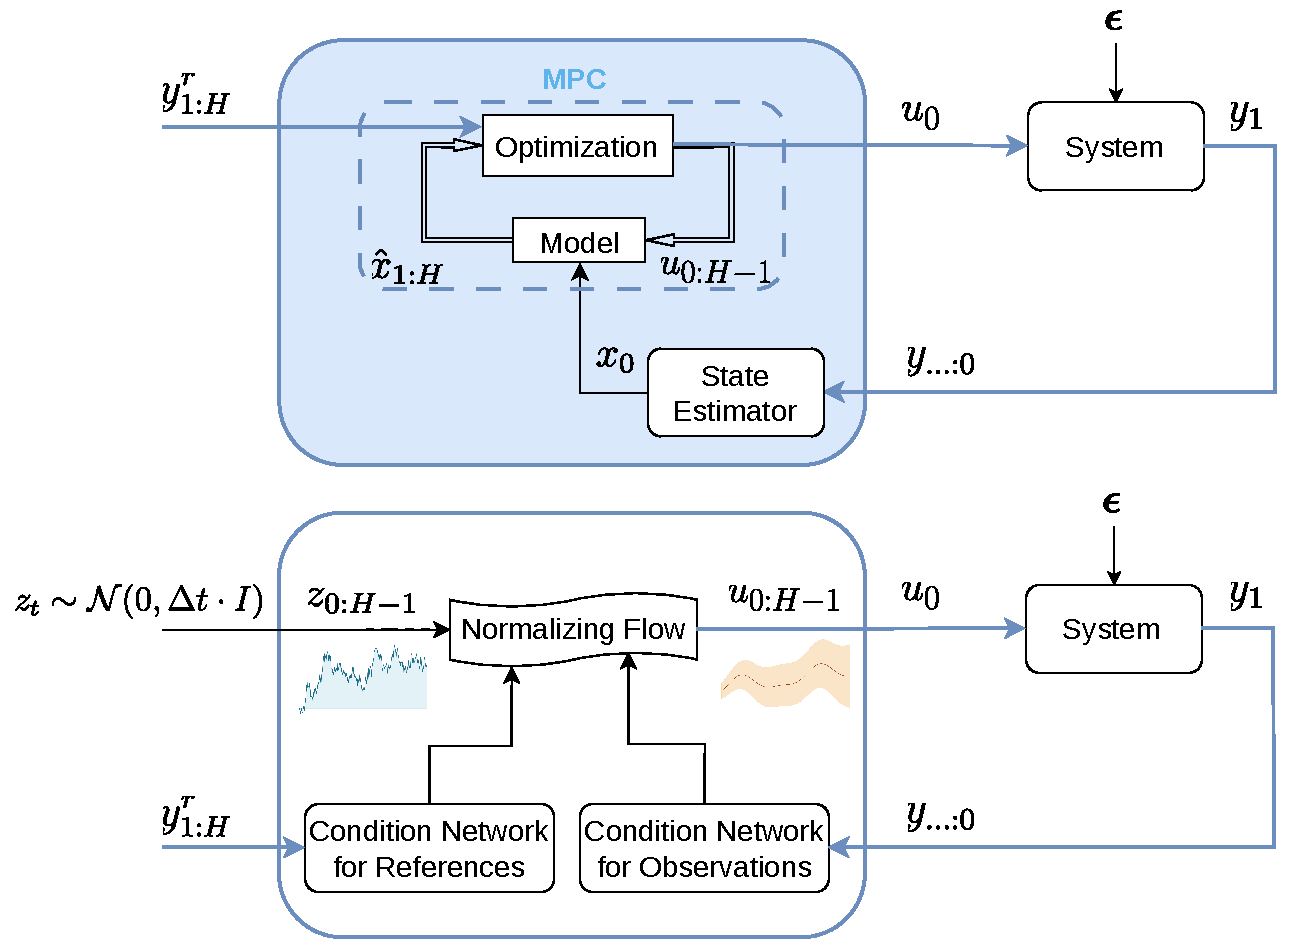
\includegraphics[width=0.8\linewidth]{figures/AmortizedSeqFlow_Control.pdf}
\caption[Amortized Sequence Flow for Control]{Applying AmortizedSeqFlow as an \ac{MPC}. The latent variable of the normalizing flow $\boldsymbol{z}_{0:H-1}$ is sampled from a Wiener process. On the other side of the normalizing flow, the target is the control input sequence $\boldsymbol{u}_{0:H-1}$. Two condition networks are applied for next-step references $\boldsymbol{y}^r_{1:H}$ and history observations $\boldsymbol{y}_{...:0}$, respectively.}
\label{fig:amortized_seq_flow_control}
\end{figure}

Comparing with the classical \ac{MPC}, AmortizedSeqFlow offers several advantages. First of all, by replacing the iterative optimization loop with a single feedforward pass through the normalizing flow, the controller has a constant execution time, which helps prevent control loop delays. Secondly, AmortizedSeqFlow integrates a state estimator with the controller, which utilizes information from history observations as much as possible. Thirdly, the normalizing flow implicitly learns the system's dynamic constraints from offline training data, ensuring that the generated control input sequences are dynamically feasible for the system to execute.

\paragraph{Validation with Lane Tracking}
We evaluated the proposed AmortizedSeqFlow as a Behavior Cloner of an MPC controller on a synthetic lane-tracking task governed by a rear-axle kinematic bicycle model. The vehicle state was $s_t=[x_t,y_t,\psi_t]$, and the steering angle $\delta_t$ was the control input. The discrete-time dynamics were

\begin{align}
x_{t+1} &= x_t+\Delta t\,v\cos\psi_t,\\
y_{t+1} &= y_t+\Delta t\,v\sin\psi_t,\\
\psi_{t+1} &= \psi_t+\Delta t\,\frac{v}{L}\tan\delta_t ,
\end{align}
with sampling time $\Delta t=0.1\,s$, constant velocity $v=8\,m\,s^{-1}$, wheelbase $L=2.7\,m$, and steering constraint $|\delta_t|\leq35^\circ$. Thus, each control step corresponded to approximately $0.8\,m$ of longitudinal travel. The lane centerlines were generated as sums of three sinusoids. Their amplitudes, spatial frequencies, and phases were sampled uniformly from $[0.15,0.9]\,m$, $[0.025,0.09]\,rad\,m^{-1}$, and $[-\pi,\pi]$, respectively. 

Training examples included recovery conditions with lateral errors sampled uniformly from $[-1.2,1.2]\,m$ and heading errors from $[-0.25,0.25]\,rad$. Expert demonstrations were produced by a constrained nonlinear MPC controller using the same nonlinear error dynamics as the evaluation plant. We generated 12,000 examples and randomly divided them into 80\% training, 10\% validation, and 10\% test sets. Each sample containes a control history of $2\,s$ and a future reference and control horizon of $1.5\,s$. Accorddingly, the AmortizedSeqFlow was trained to map a $20$ steps observation to a $15$ steps control input.

For closed-loop evaluation, we used previously unseen winding paths and simulated 300 control steps, corresponding to $30\,s$. All controllers started from a lateral error of $0.55\,m$ and a heading error of $0.12\,rad$. Performance was evaluated at lateral-measurement noise levels of $0$, $0.12$, and $0.24\,m$. The AmortizedSeqFlow controller was executed deterministically using the median latent input. We compared it with linear and nonlinear finite-horizon MPC controllers equipped with a Kalman filter. The filter observed only noisy lateral deviation and inferred the unobserved heading error through the vehicle dynamics. Identical reference paths and noise realizations were supplied to all methods.



\subsection{LatentSSMFlow in Stochastic MPC}
A stochastic \ac{MPC} relies heavily on a surrogate dynamics model to project future system behaviors over a prediction horizon $H$. When the underlying physical system is highly non-linear or exhibits multi-modal stochasticity, standard deterministic or Gaussian dynamics models fail. This method resolves this by modeling transitions using either a LatentSSMFlow or a NormFlowSDE. As shown in Figure~\ref{fig:latentssmflow_smpc}, the stochastic \ac{MPC} iteratively chooses candidate inputs $\boldsymbol{u}_{0:H-1}$ through the dynamics model to predict next-step states $\hat{\boldsymbol{x}}_{1:H}$ and select the optimal sequence that tracks a reference trajectory $\boldsymbol{y}^r_{1:H}$. 

For stochastic MPC with LatentSSMFlow, the control objective function can be written as an expectation over the stochastic state trajectories generated by the learned flow:
\begin{equation}
    J(\boldsymbol{u}_{t:t+H-1};\boldsymbol{x}_t)
    =\mathbb{E}_{\boldsymbol{x}_{t:t+H}\sim
    p_\theta(\cdot\mid\boldsymbol{x}_t,\boldsymbol{u}_{t:t+H-1})}
    \!\left[
    \sum_{h=0}^{H-1}
    \ell(\boldsymbol{x}_{t+h},\boldsymbol{u}_{t+h})
    +\ell_f(\boldsymbol{x}_{t+H})
    \right].
    \label{eq:stochastic_mpc_objective}
\end{equation}

Here, $p_\theta$ is the trajectory distribution learned by the LatentSSMFlow, $\ell$ is the stage cost function, and $\ell_f$ is the terminal cost function. The expectation is approximated by sampling multiple trajectories from the learned flow model. The optimization problem is solved using a sampling-based method, such as \ac{CEM}, a sampling-based stochastic optimization algorithm suitable for non-convex and derivative-free problems \citep{rubinstein1999cem}. At each MPC step, CEM maintains a Gaussian distribution over length-$H$ control sequences. Candidate sequences are sampled and evaluated by propagating multiple stochastic trajectories through LatentSSMFlow. The cost of each trajectory is estimated by averaging the stage and terminal costs across the sampled particles by LatentSSMFlow.

Besides, risk-aware loss and input smoothness regularization terms can be added to the cost function. In the risk term, the variance of the predicted states by LatentSSMFlow is penalized to avoid high-variance trajectories. In the smoothness term, the difference between consecutive control inputs is penalized to avoid abrupt changes in the control input sequence.

 CEM then refits its sampling distribution to the $N$ lowest-cost elite sequences. After several iterations, the control input of the optimized mean sequence over the $N$ elite sequences is applied, and the procedure is repeated at the next time step.

\begin{figure}
\centering
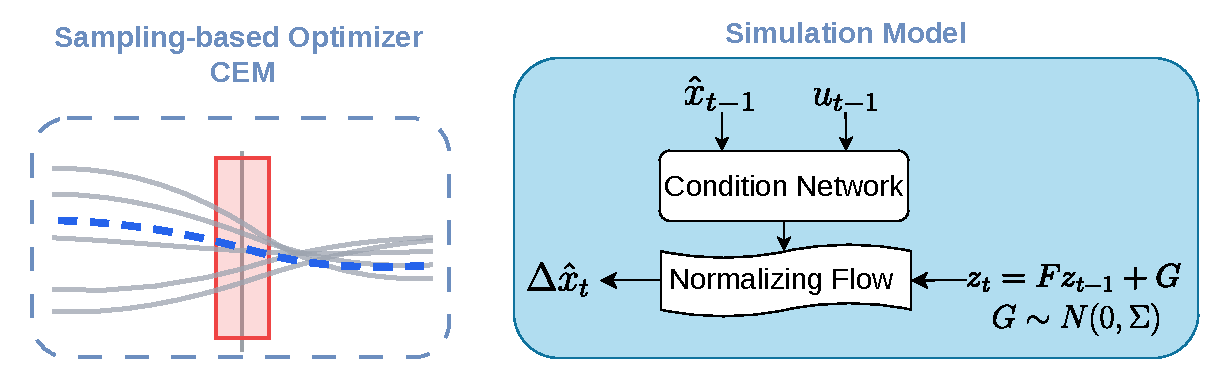
\includegraphics[width=0.8\linewidth]{figures/LatentSSM_StochMPC.pdf}
\caption[LatentSSMFlow for Control]{Application of LatentSSMFlow for the Surrogate Model in Stochastic \ac{MPC}. In LatentSSMFlow, the latent state $z_t$ propagates through linear transition equations $z_t=Fz_{t-1}+G$, where $G\sim\mathcal{N}(0,\Sigma)$ represents system noise. A Normalizing Flow maps the latent state $z_t$ back to the physical state representation $\hat{x}_t$ under the previous state $\hat{x}_{t-1}$ and input $u_{t-1}$ as conditions. A sampling-based optimization method \ac{CEM} is used to find the optimal control input.}
\label{fig:latentssmflow_smpc}
\end{figure}

\paragraph{Validation with Obstacle Avoidance}

\subsection{NormFlowSDE in MPPI}
\ac{MPPI} is a sampling-based stochastic \ac{MPC} method that estimates the optimal control update from a path integral rather than differentiating the dynamics or the cost function \citep{williams2017mppi}. This property makes it particularly suitable for NormFlowSDE: the learned model already generates continuous-time stochastic state paths by numerical integration, and these paths can be used directly as the Monte Carlo rollouts required by MPPI. Thus, the same model represents both the nonlinear mean dynamics and the non-Gaussian process uncertainty considered during control.

\paragraph{Learning the controlled dynamics}
For control, Equation~\ref{eq:flow_sde} is adapted by conditioning both the drift and the flow-based stochastic increment on the control input:
\begin{equation}
    d\boldsymbol{x}_t
    = f_\varphi(\boldsymbol{x}_t,\boldsymbol{u}_t,t)\,dt
    + g_\phi(\boldsymbol{\epsilon};
        \boldsymbol{x}_t,\boldsymbol{u}_t,t)\sqrt{dt},
    \qquad
    \boldsymbol{\epsilon}_t\sim\mathcal{N}(\boldsymbol{0},\boldsymbol{I}).
    \label{eq:controlled_normflowsde}
\end{equation}
Here, $f_\varphi$ learns the conditional drift, whereas the invertible normalizing flow $g_\phi$ transforms Gaussian distribution into state- and input-dependent stochastic increments. The stochastic term can model complex uncertainty and also the unmodeled dynamics residual. 

The model is trained offline from states and inputs trajectories $\mathcal{D}=\{(\boldsymbol{x}(t),\boldsymbol{u}(t))\}$, which can be collected from the real system or a high-fidelity simulator. A two-stage training procedure is used: first, the drift network $f_\varphi$ is trained to minimize the one-step prediction error using \ac{MSE}, and then the flow network $g_\phi$ is trained together with the drift network using the loss function Eq.~\ref{eq:normflowsde_loss}. After training, the NormFlowSDE model can be applied in an \ac{MPPI} framwork. During deployment, the current state initializes the SDE solver, and sampled trajectories generate an ensemble of possible future paths for every candidate input sequence.

\paragraph{Model Predictive Path Integral control}
At control time $t$, MPPI maintains a nominal sequence
$\boldsymbol{U}_t=(\boldsymbol{u}_t,\ldots,\boldsymbol{u}_{t+H-1})$ over a horizon $H$. It draws $K$ perturbation sequences
$\delta\boldsymbol{U}_t^{(k)}$, commonly from a zero-mean Gaussian distribution with covariance $\boldsymbol{\Sigma}_u$, and forms the candidate inputs
\begin{equation}
    \boldsymbol{u}_{t+h}^{(k)}
    =\Pi_{\boldsymbol{U}}\!\left(
    \boldsymbol{u}_{t+h}+\delta\boldsymbol{u}_{t+h}^{(k)}\right),
    \qquad h=0,\ldots,H-1,
\end{equation}
where $\Pi_{\boldsymbol{U}}$ enforces the feasible input set. Each candidate is integrated through Equation~\ref{eq:controlled_normflowsde}. With $M$ independent dynamics realizations per candidate, its expected trajectory cost is approximated by
\begin{equation}
    \widehat{J}_k
    =\frac{1}{M}\sum_{m=1}^{M}\left[
    \sum_{h=0}^{H-1}
    \ell(\boldsymbol{x}_{t+h}^{(k,m)},
         \boldsymbol{u}_{t+h}^{(k)})
    +\ell_f(\boldsymbol{x}_{t+H}^{(k,m)})
    \right]+\mathcal{C}_{\text{MPPI}}^{(k)},
    \label{eq:normflowsde_mppi_cost}
\end{equation}
where $\ell$ and $\ell_f$ are the running and terminal costs. The term
$\mathcal{C}_{\text{MPPI}}^{(k)}$ denotes the importance-sampling correction associated with perturbing the nominal control distribution; it also incorporates the quadratic control penalty in the standard MPPI formulation. State and obstacle constraints can be included as soft penalties in $\ell$ or as an infinite cost for invalid rollouts. Thus, $\widehat{J}_k$ is the Monte Carlo estimate of the objective $J(\boldsymbol{U}_t^{(k)};\boldsymbol{x}_t)$ for the $k$-th perturbed control sequence, augmented by the MPPI sampling correction.

The path costs are converted into normalized importance weights,
\begin{equation}
    w_k=\frac{\exp[-(\widehat{J}_k-\rho)/\lambda]}
    {\sum_{j=1}^{K}\exp[-(\widehat{J}_j-\rho)/\lambda]},
    \qquad \rho=\min_j\widehat{J}_j,
    \label{eq:normflowsde_mppi_weights}
\end{equation}
where the subtraction of $\rho$ improves numerical stability and the temperature $\lambda>0$ controls selectivity. A small $\lambda$ concentrates the update on the lowest-cost paths, whereas a large $\lambda$ averages more broadly over the sampled candidates. The nominal controls are then shifted toward perturbations that generated low-cost trajectories:
\begin{equation}
    \boldsymbol{u}_{t+h}\leftarrow\boldsymbol{u}_{t+h}
    +\sum_{k=1}^{K}w_k\delta\boldsymbol{u}_{t+h}^{(k)},
    \qquad h=0,\ldots,H-1.
    \label{eq:normflowsde_mppi_update}
\end{equation}

Only the first optimized input is applied to the plant, as the other receding-horizon control frameworks. At the next environment step, the horizon is shifted, the terminal input is initialized, and the sampling-and-integration procedure is repeated using the new state estimate. This receding-horizon feedback corrects model error and newly observed disturbances.

The integral form of NormFlowSDE is especially useful here. For each candidate control sequence, an SDE solver computes complete stochastic paths rather than only point predictions. MPPI then approximates its path integral with the same ensemble, so no additional uncertainty propagation or local linearization is required. The candidate and uncertainty rollouts are mutually independent and can be evaluated in parallel. Moreover, risk sensitivity and input smoothness can also be introduced.

\begin{figure}
\centering
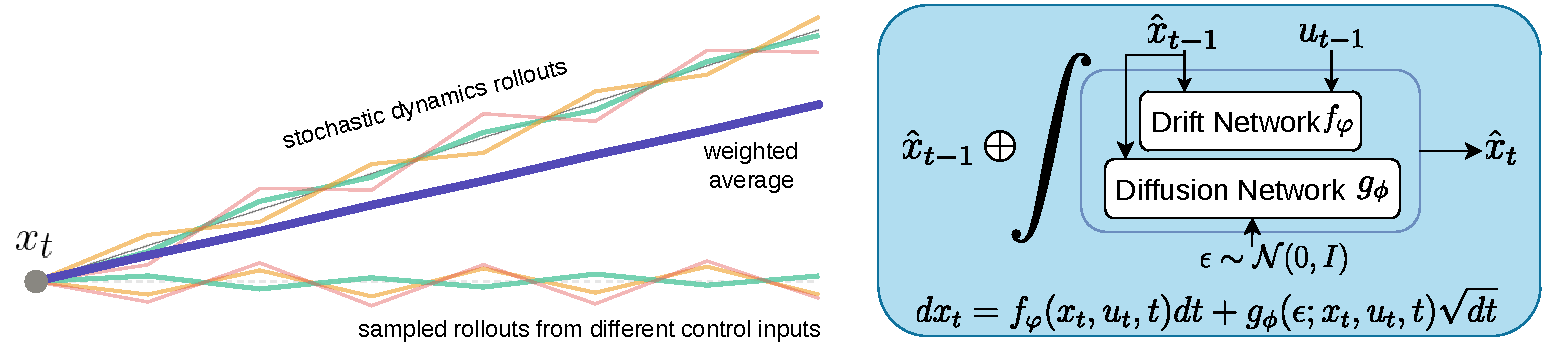
\includegraphics[width=\linewidth]{figures/NormFlowSDE_MPPI.pdf}
\caption[NormFlowSDE for MPPI]{NormFlowSDE as the probabilistic surrogate model in MPPI. Perturbed candidate control sequences are integrated through the learned controlled SDE to produce stochastic state trajectories. Their path costs determine importance weights, which update the nominal control sequence before the first input is applied in receding-horizon form.}
\label{fig:normflowsde_mppi}
\end{figure}

\paragraph{Validation with Navigation Task}


\subsection{CondStochInterpolant in DDPO}
The CondStochInterpolant control policy generates action chunk based on history observations and current state, as shown in Figure~\ref{fig:condstochinterpolant_control}. At the beginning of environment step $t=0$, the agent retrieves the sliding window of historical observations $O_{...:0}$. A condition network $C_\psi$ embeds these temporal observations into a low-dimensional embedding vector $c$, which provides context information for the generative process of the stochastic interpolant. Unlike the CondStochInterpolant proposed for state estimation, where the inferred coarse trajectory in the latent space provides an informative basis for state estimation, they do not necessarily provide a direct mapping to the action chunk. Thus, the latent space $\mathcal{U}_0$ here is chosen to be a standard Gaussian distribution and is transformed into a high-fidelity action chunk $\mathcal{U}_1$ by numerically integrating the \ac{SDE} from $\tau = 0$ to $\tau = 1$:
\begin{equation}
    d\mathcal{U}_\tau = \left[ v_\varphi(\mathcal{U}_\tau, \tau; c) + g_0^2 S_\phi(\mathcal{U}_\tau, \tau; c) \right] d\tau + g_0 \sqrt{2\sigma_\tau} dW_\tau.
\end{equation}

The agent generates an action chunk $a_{0:H-1}$ in closed loop. Taking the actions, the environment updates the new observations $O_{1:H}$. To update the networks ($\varphi, \phi, \eta, \psi$) online using \ac{RL}, the generated action chunks are evaluated against a reward function $r$, which also considers the history and updated observations.


\begin{figure}
\centering
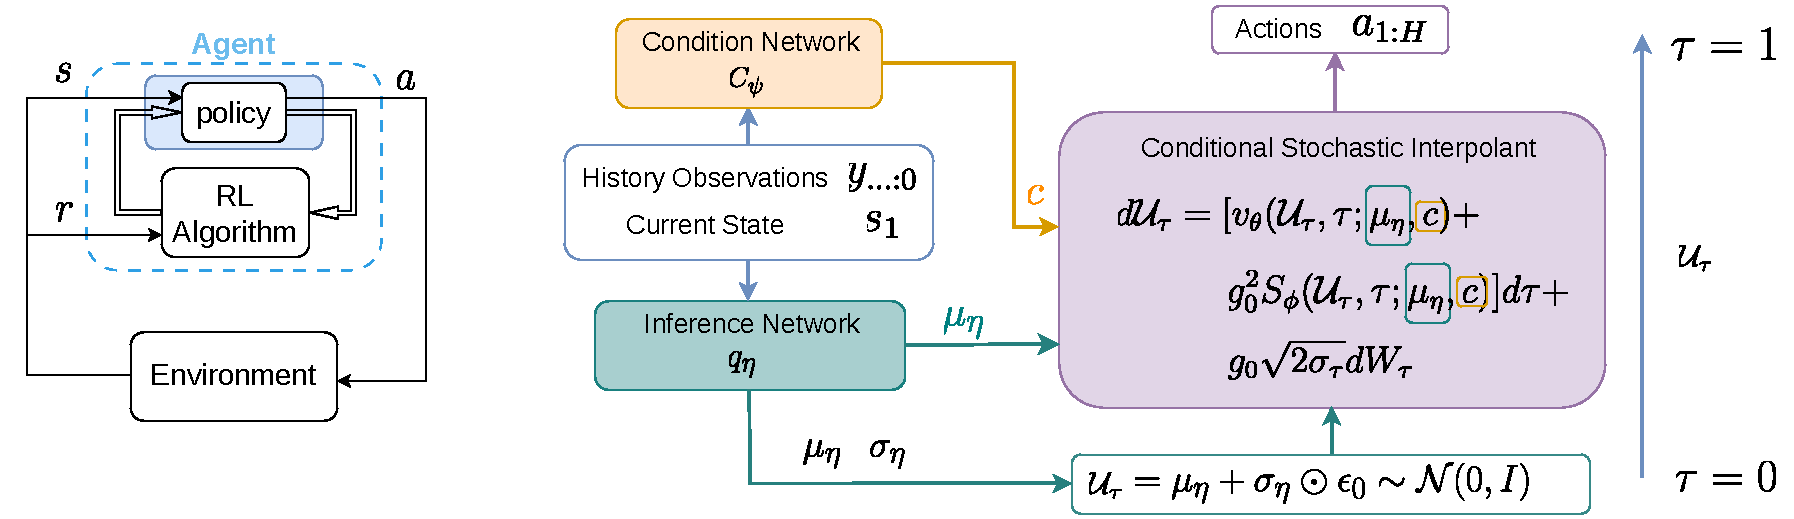
\includegraphics[width=\linewidth]{figures/CondStochInterpolant_Control.pdf}
\caption[CondStochInterpolant for Control]{Closed-loop reinforcement learning agent utilizing a Conditional Stochastic Interpolant policy for action chunk generation. At timestep $t=1$, the policy processes past observation history $O_{...:0}$ and the condition network $C_\psi$ maps these conditions to a context embedding $c$. The policy integrates an \ac{SDE} from an initial state $\mathcal{U}_0$, which samples a standard Gaussian distribution. The \ac{SDE} is driven by a velocity network $v_\varphi$ and a score network $S_\phi$. Both networks are conditioned on the context embedding $c$. At flow time $\tau=1$, the integrated trajectory yields the final, smooth action chunk $a_{1:H}$, which is then executed in the environment.}
\label{fig:condstochinterpolant_control}
\end{figure}

\paragraph{Validation with Robotic Manipulation Task}
